\chapter{Design Realization} \label{ch:designRealization}
As the requirements are derived and the development platform is chosen, the system presented in \autoref{ch:overview} may be designed. Evaluating the concept design from \autoref{ch:overview} it is seen that the concept has four bands-pass filters and one high-pass that need to be designed.


\section{Practical Design Considerations}

Before designing the band-pass filters, RMS analysis, and compressor, practical design considerations needs to be done, as designing and simulating the system do not mean the system can be implemented because of hardware constraints. In this section following topics will be covered:

\begin{itemize}
\item[•] Phase response and group delay.
\item[•] Filter types.
\item[•] Computational constraints.
\end{itemize}

As the signal needs to be reconstructed in the end of the system, it is desirable that the reconstructed signal do not have frequency bands which are out of phase compared to the original input signal. If the bands are out of phase the resulting sound may be unpleasant to listen to. Therefore a design requirement to the system is to ensure that the signals from each band are added together without changing the relative phase between each band.


\subsection*{Phase response and group delay}
One of properties in non-statical filters such as low-pass and band-pass filters are the phase shift. For a filters such as the Butterworth low-pass filter, the phase shift begins at the frequency at one decade below the cutoff frequency and ends one decade above. The phase shift in-between for most analog filter except Bessel filter, have a non-linear phase response. Because of the phase response is non-linear, the group-delay will likewise not be linear as seen in \autoref{fig:groupDelayIirPrev}.

\begin{figure}[H]
\centering
\begin{subfigure}[t]{0.435\textwidth}
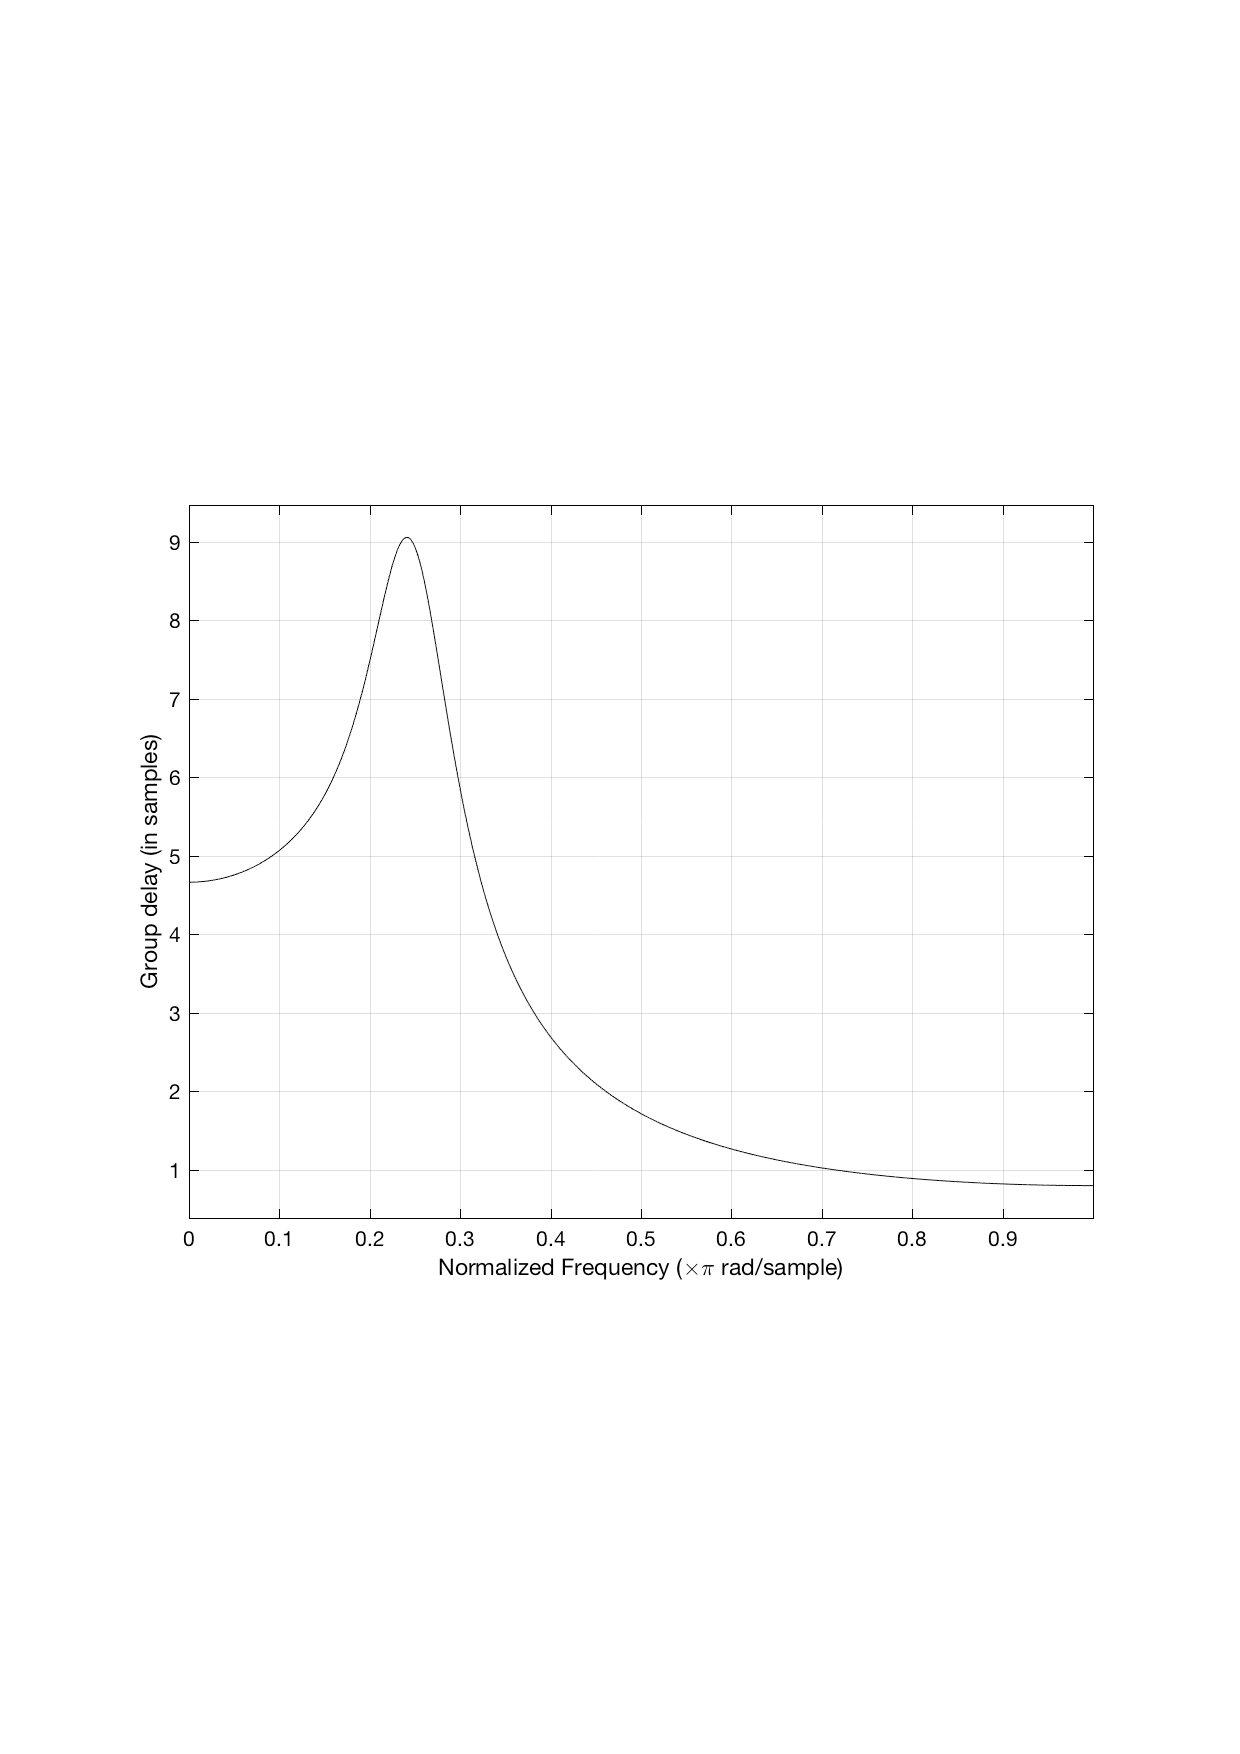
\includegraphics[width=\linewidth]{groupDelayIirPrev}
	\caption{Group delay of a 4th order IIR filter.}
	\label{fig:groupDelayIirPrev}
\end{subfigure}
\hspace{6mm} 
\begin{subfigure}[t]{0.47\textwidth}
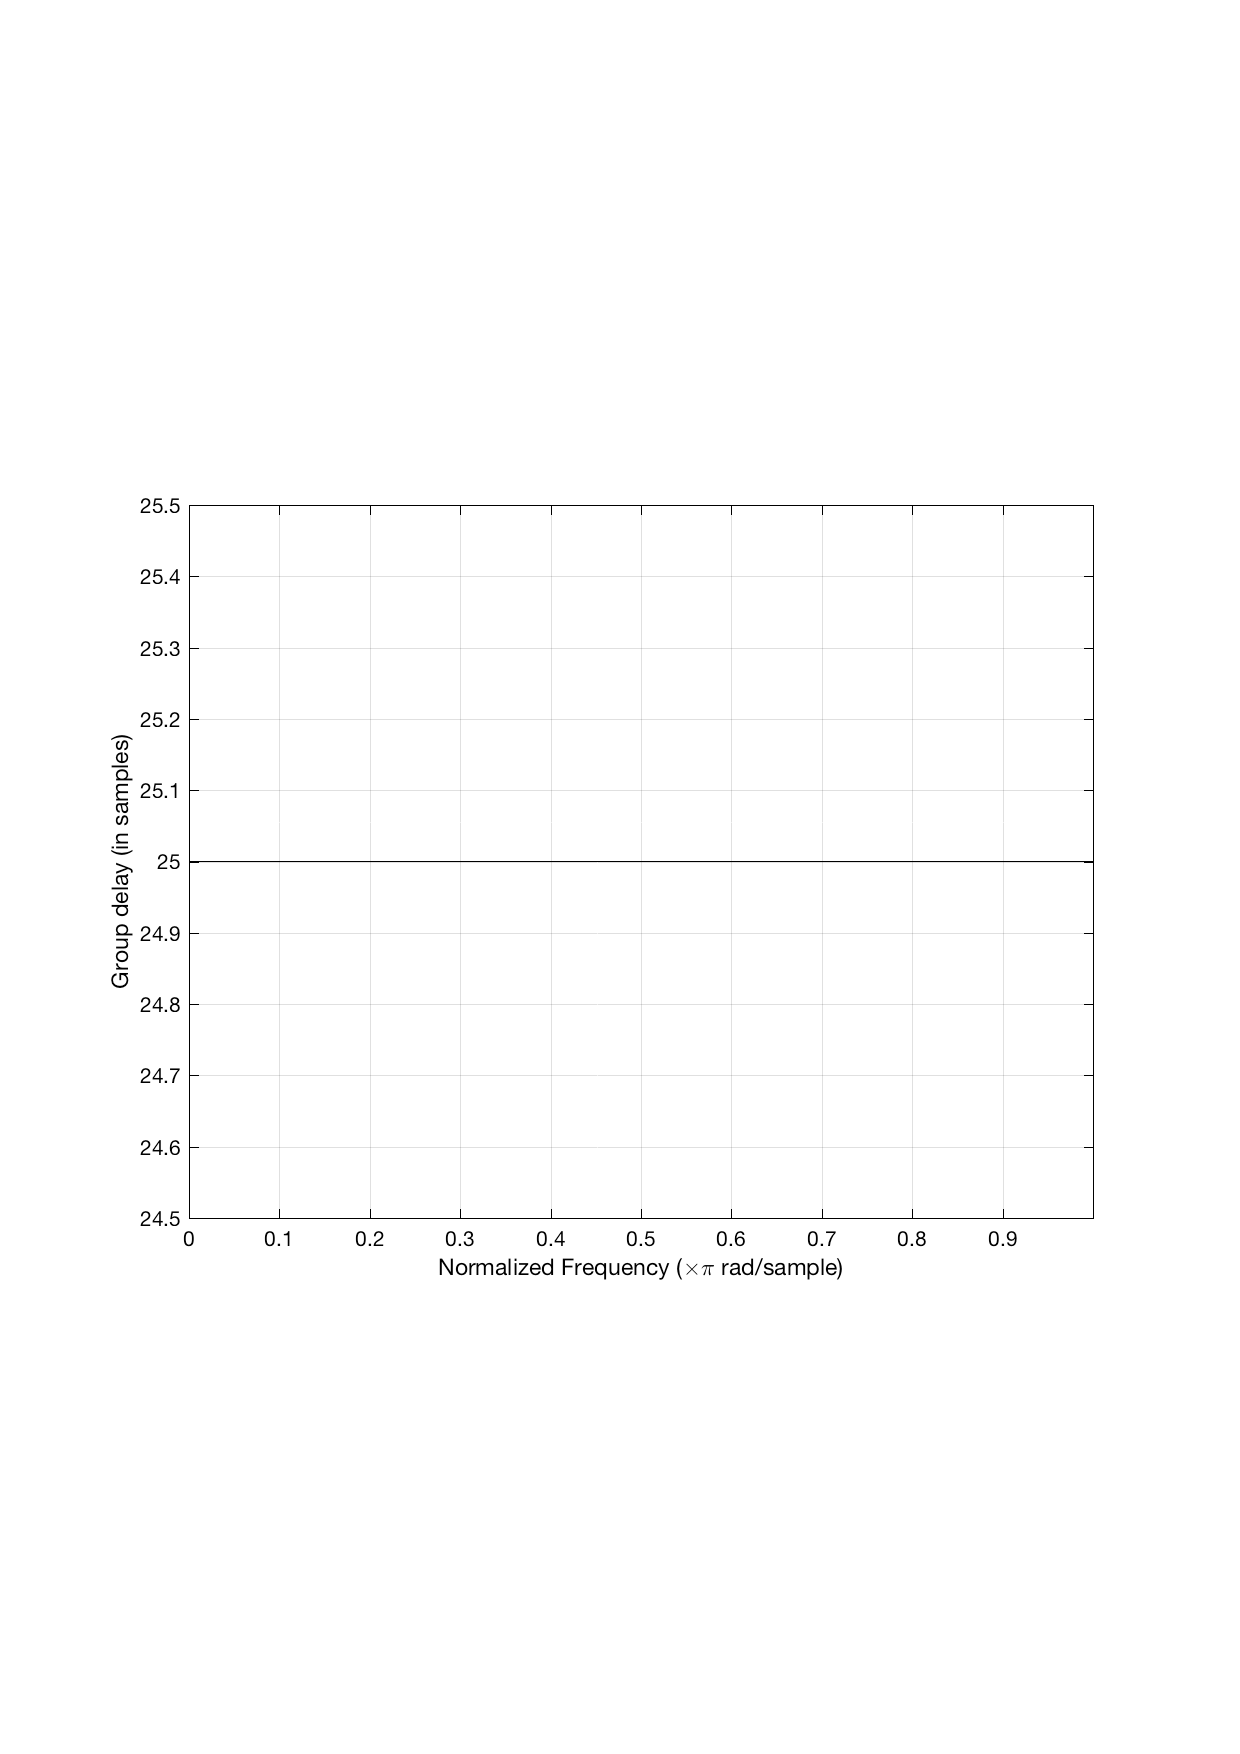
\includegraphics[width=\linewidth]{groupDelayFirPrev}
	\caption{Group delay of a 50th order FIR filter.}
	\label{fig:groupDelayFirPrev}
\end{subfigure}
\caption{Group delay of IIR and FIR filter.}
\label{fig:filterGroupDelay}
\end{figure}

The group delay is an important parameter to take into account, as it specifies the sample delay for each frequencies. 1 sample delay is equivalent to 20.83 $\mu$s in a 48 kHz system. \autoref{fig:groupDelayIirPrev} shows that the group delay for IIR filters is non-linear with a peak at the normalized frequency 0.25 $\pi rad$. To calculate the time delay at 0.25 $\pi$ rad following expression can be used:

\begin{equation}
t_{d}= \frac{n_{s}}{f_s}
\end{equation}

Where $n_{s}$ is the number of samples delayed and $f_s$ is the sampling rate. A non-linear group delay will be hard to compensate compared to a constant group delay, thus a constant group delay is desirable. To achieve a constant group delay a linear phase filter needed as the phase response is linear. Linear phase can be found in FIR filters and Bessel filters. Because of the constant group delay in linear phase filter, it eases the design as constant delays can be implemented to compensate the phase shift in filters. Because the Bessel filter do not have a very sharp cutoff compared to other filter types, a high order Bessel filter will be needed. A high order IIR however has risk of being unstable. FIR filters are therefore chosen as they have all the required properties and do not get unstable.


\subsection*{Computational Constraints}
Another subject to consider is the constraints regarding computational power to perform filter algorithms. For FIR filters the amount of instructions to compute the filter output increases by the filter order, as calculating each tap in the filter is equal to a multiply and accumulate. Therefore even though a very high order filter in theory is realizable, the computational constraint needs to be considered. 

The performance of the DSP is 100 MIPS. At a sample rate of 48 kHz, this will result in approximately 2083 instructions available in-between each sample. A 3000 order FIR filter for instance is thus not realizable on the platform with a sampling rate on 48 kHz as the DSP will not finish calculating the filter output in time before next sample. Designing FIR filters will therefore be difficult as the cutoff frequencies for all required filters are very low relative to the sampling rate. A cutoff frequency located far from the sampling rate results in a long impulse response for a FIR filter. To a achieve a steep cut more samples of the impulse response are needed thus increasing the order of the filter. 

\subsection*{Multirate signal processing with Multistages}
A solution to avoid very high order filters is to downsample the signal into a signal with a lower sampling rate. By downsampling the signal the impulse response of an equivalent FIR filter at the same cutoff frequency is shortened and the amount of taps is therefore reduced. To downsample however requires an anti-aliasing filter to avoid aliasing. The order of the anti-aliasing filter should be high enough to attenuate frequencies above the new $fs/2$. Also the cutoff frequency may still be very low. 

To minimize the order of the anti-aliasing filters and amount of instruction to perform signal processing, the signal is downsampled by a factor of 2 until the lowest required band is achieved. An example and explanation of why a downsampling factor of 2 is more efficient than high downsampling factors is now explained. 

A high downsampling factor e.g. 32




By doing so the filter order for each anti-aliasing filter is kept low as the cutoff frequency of each band is closer to the sampling frequency. Also, the whole bandwidth of the audio signal is split into octave bands which is an advantages if an equalizer and spectrum analyser are desired.

Applying the considerations to the system, following new overall system may be presented.

\begin{figure}[H]
\centering
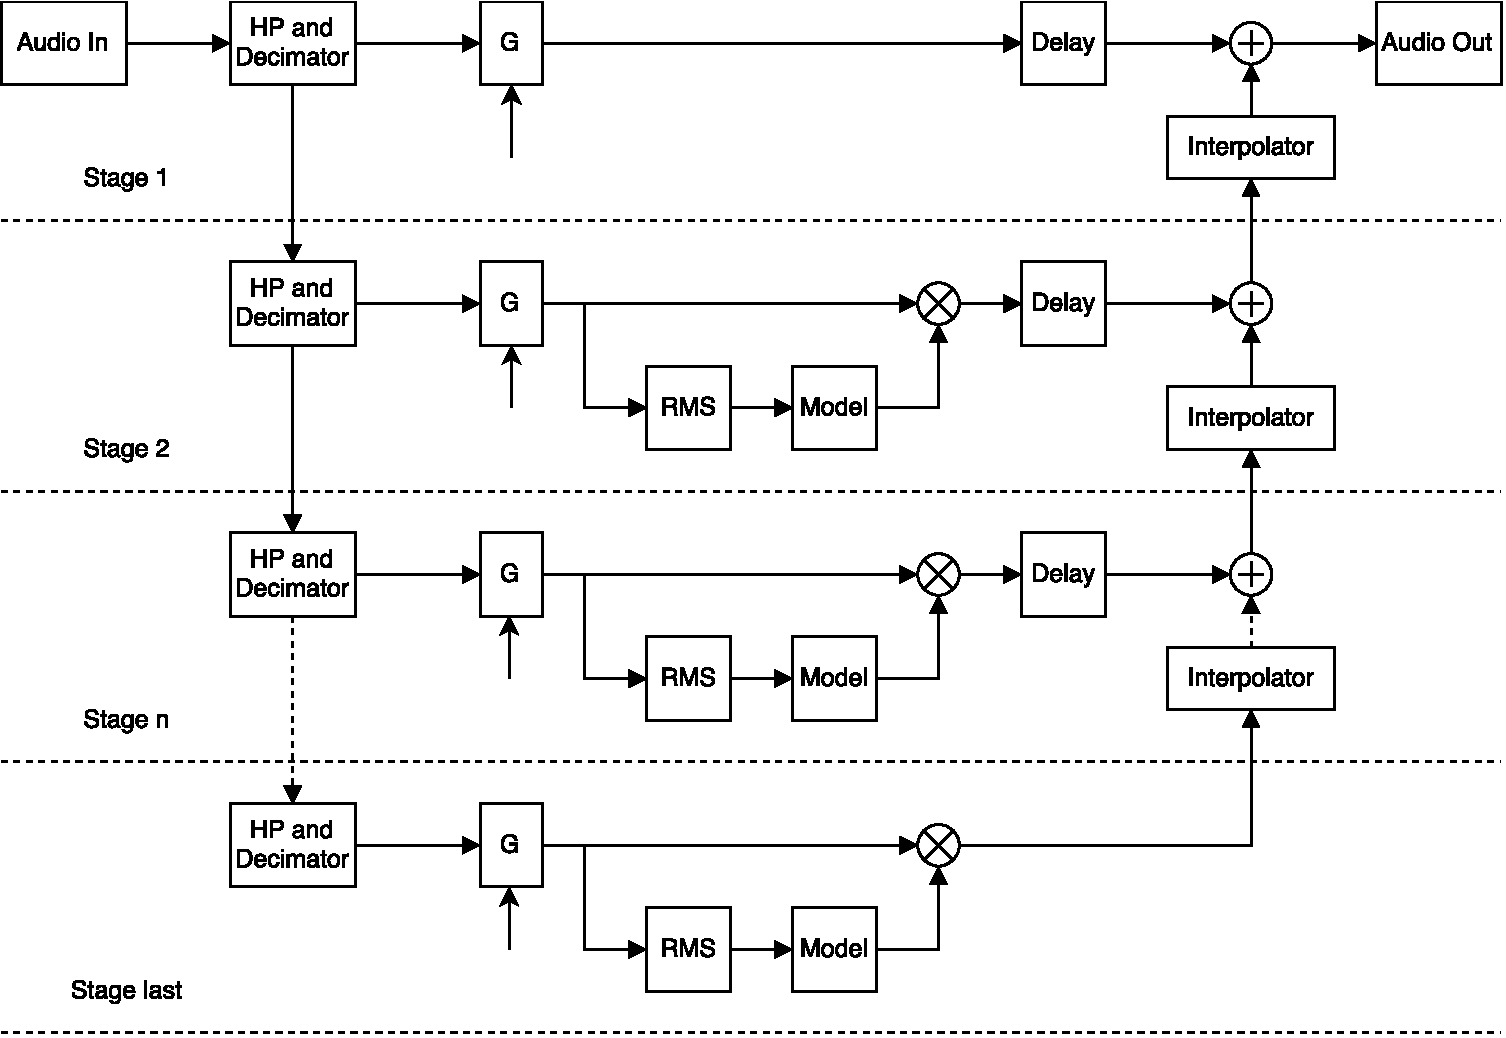
\includegraphics[width=0.75\textwidth]{figures/designRealBlock1.pdf}
\caption{Overall system with practical considerations.}
\label{fig:designRealBlock}
\end{figure}




In comparison to previous system overview decimation, "HP and Decimator" and "interpolator" blocks are added to the system. The design of these blocks including the RMS and model will discussed in following sections.

\todo{Husk at tilføje at vi anvender 8 baand.}

\section{High-Pass filter and Decimator}

A decimator is, as previously mentioned, a subsystem consisting of an anti-aliasing filter and a downsampler. If the signal is a combination of high and low frequencies, the anti-aliasing filter, filters high frequencies to avoid aliasing when downsampling. As the anti-aliasing essentially is a low-pass filter the chosen design choice takes advantages of the low-pass, so the remaining filter to be designed is a high-pass filter. By using a design technique called spectral inversion, a high-pass filter can be designed by subtracting the output of the anti-aliasing low-pass filter from the input signal. By doing so, a high pass filter is saved from the system. The decimation block is seen in figure \autoref{fig:designRealDecimator}.

\begin{figure}[H]
\centering
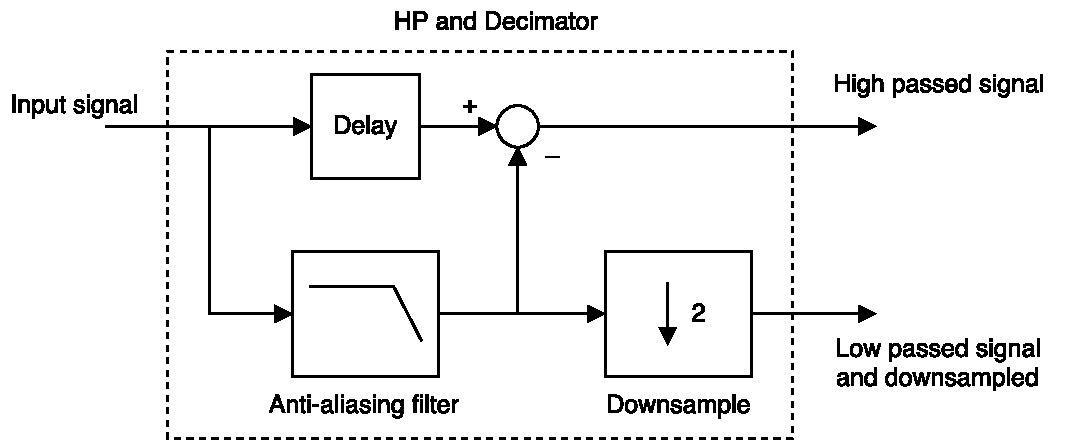
\includegraphics[width=0.75\textwidth]{figures/designRealDecimator.pdf}
\caption{The decimation block consist of a decimator and a spectral inversion to achieve a high-pass filter.}
\label{fig:designRealDecimator}
\end{figure}

To apply spectral inversion to achieve a high-pass filter, it required to apply a delay of the input signal before subtraction. This is due to the group delay of the anti-aliasing filter, and to apply spectral inversion, the phase between the signal must be intact.


\section{Interpolator}

Opposite to the decimator is the interpolator. As it is desired to reconstruct the signal, upsampling is applied to the downsampled signal. To upsample the downsampled signal, zeros are added to the signal. Since the upsampling factor is 2, a zero is added in-between each sample. This adds high frequency components noise which is then filtered by using a low-pass filter. In this case the same anti-aliasing filter from the decimator is sufficient. The block diagram of the interpolator is seen in \autoref{fig:designRealInterpolator}.

\begin{figure}[H]
\centering
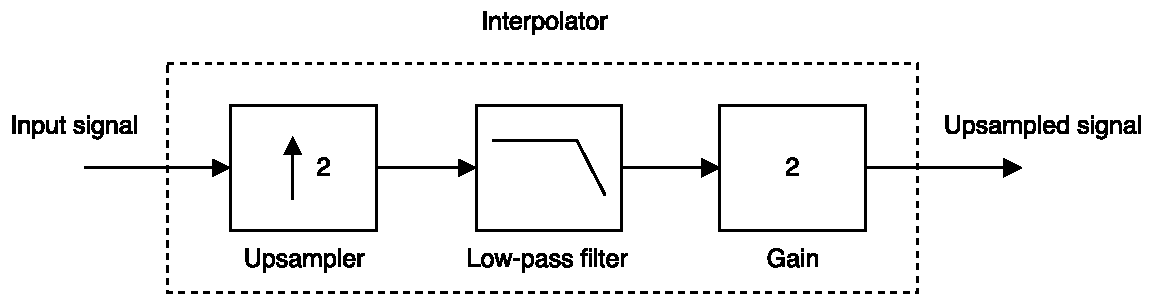
\includegraphics[width=0.75\textwidth]{figures/designRealInterpolator.pdf}
\caption{The interpolator consist of a upsampler, low-pass filter and a gain factor determined by the upsampling factor.}
\label{fig:designRealInterpolator}
\end{figure}

Applying the low-pass filter smooths the signal, but because every second sample is zero a gain of a factor of 2 needs to be applied to normalize the signal.


\section{RMS and Model}

To design a RMS limiter a RMS analysis and a mathematical function describing the gain are needed. The input signal from a band is fed in parallel, into a RMS block, which calculates the RMS-value as the output. The output is sent to a "Model" block which essentially checks if the RMS value is above a threshold. If the RMS-value is above the threshold the "Model" will apply a gain derived from a mathematical expression to the band signal to attenuate it. If the RMS-value is below, the output will be a unity gain. The block digram of the RMS and model is seen in \autoref{fig:designRealRMS}.

\begin{figure}[H]
\centering
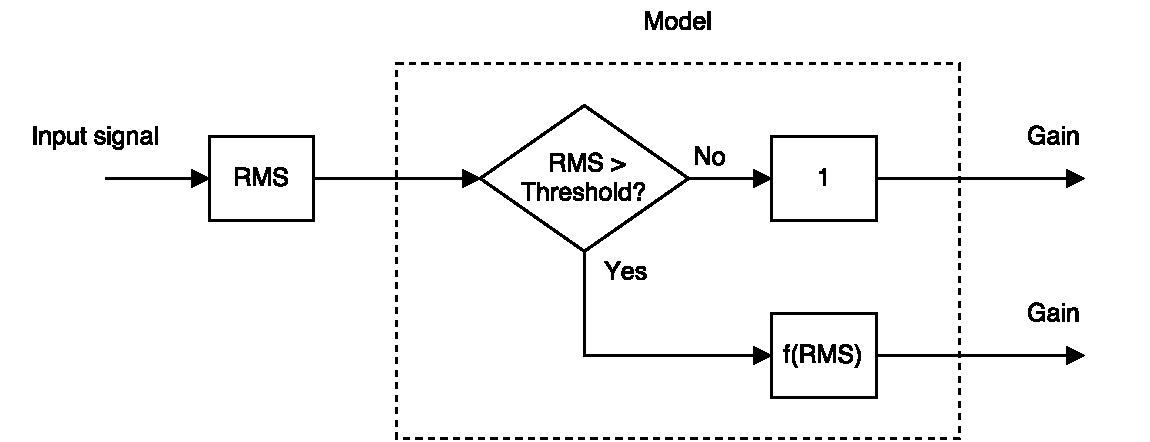
\includegraphics[width=0.75\textwidth]{figures/designRealRMS.pdf}
\caption{The RMS-value is first calculated and then fed into a subsystem that determines which gain to apply on the band signal.}
\label{fig:designRealRMS}
\end{figure}

To determine the threshold of the "model", a test of the loudspeaker needs to be done. The purpose of the test is to examine at which RMS-level the loudspeaker is either performing bad or damaging itself. To perform a RMS-analysis the minimum aount of samples needed is the amount of samples to represent the lowest frequency in that band. This introduces a small attact time, meaning the RMS-limiter cannot catch fast transients.



\section{Complete system}

The RMS limiter cannot protect the loudspeaker againt transients such as kicks in music and short spikes due to the small attack time. To avoid potential damage, a peak limiter is inserted in the upsampled 530 Hz band. The threshold of this limiter is set very high, as the main purpose it to protect the loudspeaker at cases where the RMS-limiter is not fast enough to respond. Another RMS-limiter is inserted in the upsampled 530 band. Because the signal is split into 4 bands, the 530 Hz band RMS-limiter ensures that the upsampled signal below 530 Hz do not exceed the threshold.

\begin{figure}[H]
\centering
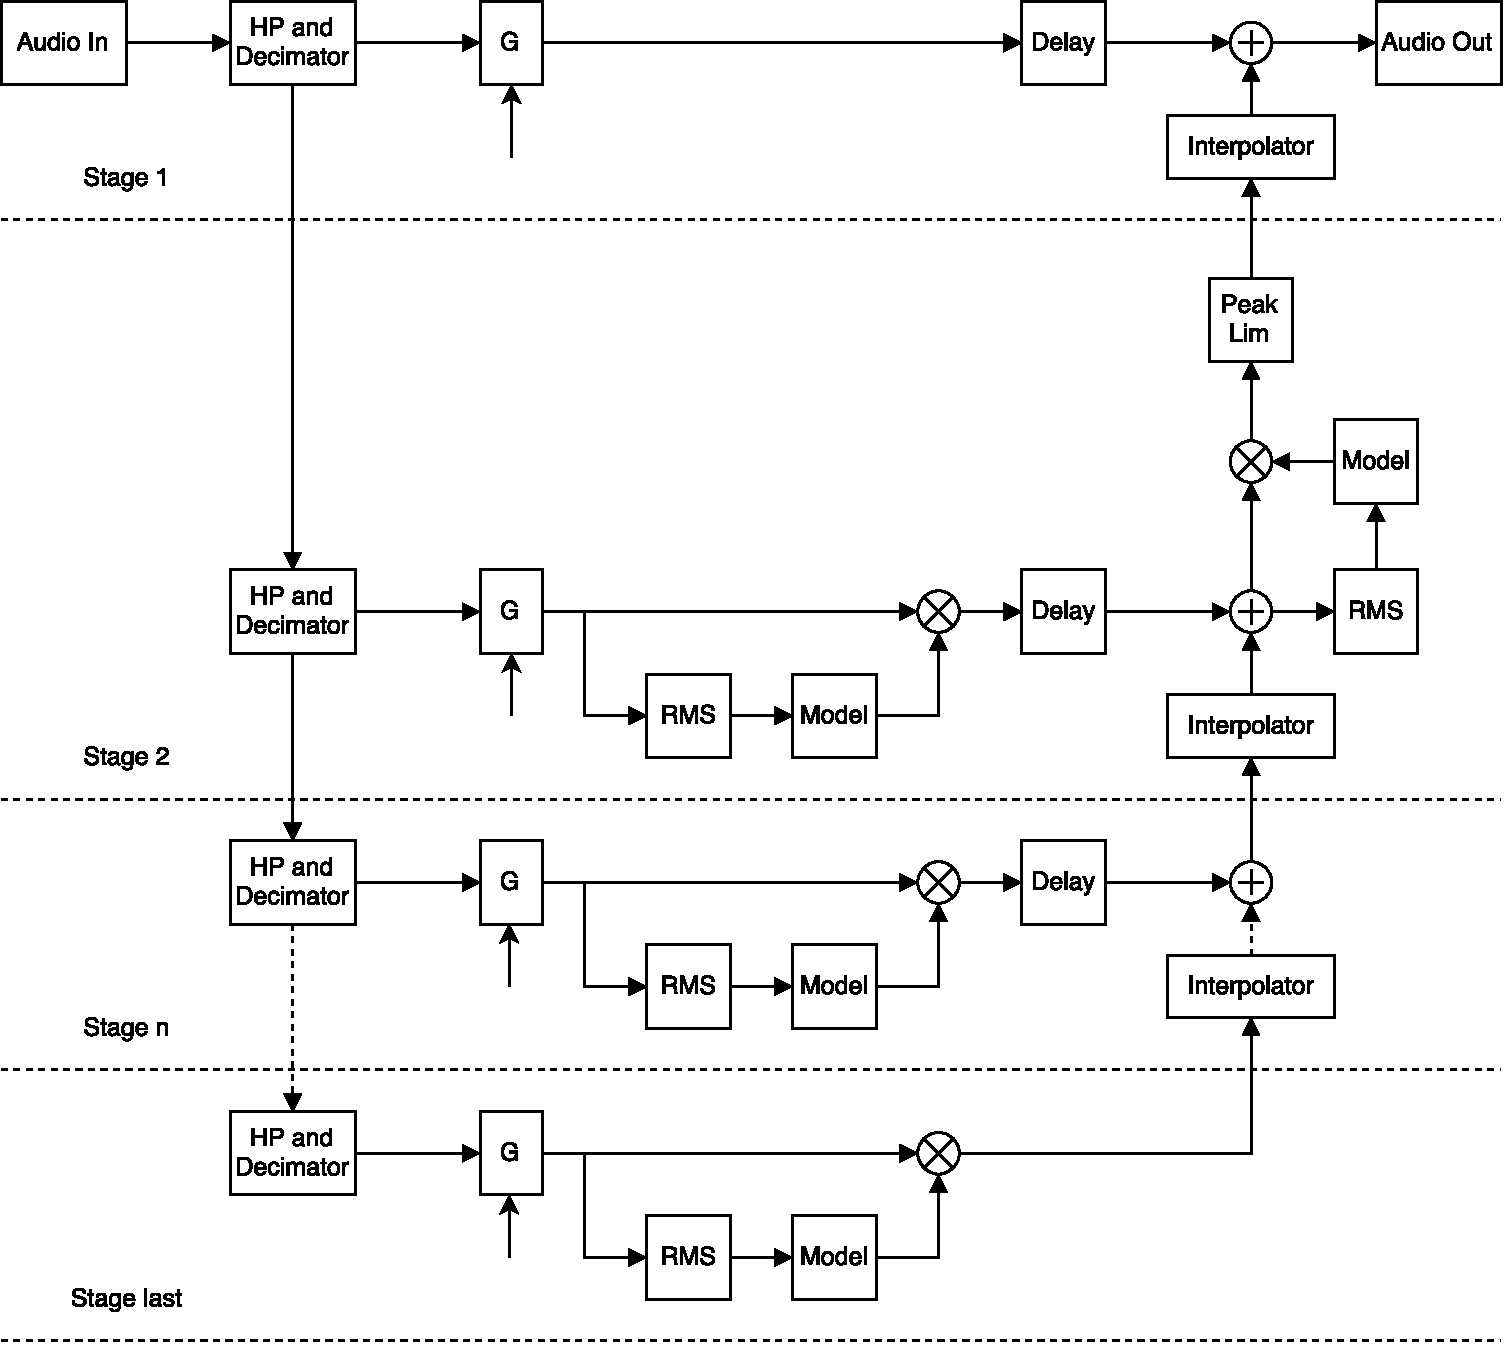
\includegraphics[width=0.75\textwidth]{figures/designRealFull.pdf}
\caption{The complete overall system to be designed.}
\label{fig:designRealBlock}
\end{figure}

The complete system is now explained and each subsystem of the system may now be designed in the following chapters.
